% Computer Architecture (4190.308) Fall 2016 
% Seoul National University CARES Lab
% Lab 2 documentation

% Lines that need modification : 27~29

\documentclass{article}
\usepackage{graphicx, caption, subcaption, verbatim, moreverb, alltt, algorithm2e, kotex}
\usepackage[protrusion=true,expansion=true]{microtype}
\usepackage{fancyvrb}
\let\verbatiminput=\verbatimtabinput

\setlength{\oddsidemargin}{0.25in}	% 1.25in left margin 
\setlength{\evensidemargin}{0.25in}	% 1.25in left margin (even pages)
\setlength{\topmargin}{0.0in}		% 1in top margin
\setlength{\textwidth}{6.0in}		% 6.0in text - 1.25in rt margin
\setlength{\textheight}{9in}		% Body ht for 1in margins
%\setlength{\parindent}{0pt}			% do not indent the begining of paragraph
\addtolength{\topmargin}{-\headheight}	% No header, so compensate
\addtolength{\topmargin}{-\headsep}	% for header height and separation


% type user-defined commands here

\begin{document}

\title{Lab 2: Pipelined Barrel Shifter}   % type title between braces
\author{CSE 4190.308 Computer Architecture \\ 2 Exercises (Total 80 Points)}
\date{Received: March 19, 2016 \\Due: 11:00 a.m., March 28, 2016\\ \ \\ TA Office Hours: 7:00 - 8:00 p.m., 3/25, 3/26, 3/27} 
\maketitle

\section{Introduction}
In the last lab, we implemented a Barrel Shifter from gates. 
In this lab, we will extend the Barrel Shifter implementation to support the left shift (\texttt{<<}) operation. 
We will then create a pipelined implementation of the Barrel Shifter.

Pipelining is an important technique in hardware design. 
As combinational circuits grow in functionality and complexity, 
the number of gates delays needed to compute the result of the circuit.
Long combinational paths can seriously impact the operating frequency of the circuit. 
As a result, circuit designers introduce registered pipeline stages to cut these combinational paths. 
This improves the clock frequency, but adds latency to the design, since results take an extra cycle to compute.
However, if each pipeline stages can be used simultaneously, the throughput of the design can increase, despite the increased latency.
Figure 1 shows a pipelined Barrel Shifter. Notice that both data and control must be pipelined.

\subsection{Lab Organization}
The first part of the Lab 2 consists of extending the combinational Barrel Shifter 
that you built in Lab 1 to implement left shift, and then pipelining the design.

\begin{figure}[hb]
	\centering
	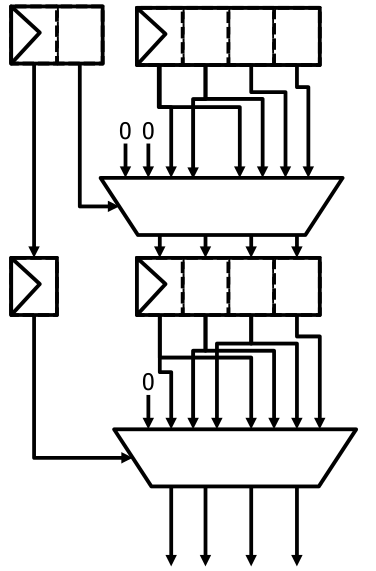
\includegraphics[width=0.3\linewidth]{pipeBS.png}
	\caption{A pipelined, 4-bit Barrel Shifter}
	\label{fig:pipelined_brs}
\end{figure}

\section{Getting Started}
\subsection{How to Download the Source Code}
% As we memtioned before, every assignments on this course will be managed in our svn server.
% You can get the skeleton source codes of Lab 2 by executing the script file \texttt{add-lab2.sh}
% which can be found on the course web page. Put the script in upper directory of your assignment directory named as your ID.
Lab 2의 실습 코드를 받는 방법은 기존 Lab들과 동일합니다.
수업 홈페이지에 올라와 있는 \texttt{add-lab2.sh} 스크립트를 다운받고,
이전 Lab을 수행했던 실습 디렉터리의 상위에 위치시킵니다.

\begin{Verbatim}[frame=single]
   $ ls
   add-lab2.sh YOUR_ID/
   $ ls YOUR_ID/
   lab0/ lab1/
\end{Verbatim}

% The script file receives an ID as its first argument.
% You should give your own ID you've created before using the \texttt{student-create.sh} script.
% A password of archi13 can be required while you executing the script.
% It is the same password with the one of our course web page.
그 후 아래 예제와 같이 본인의 ID를 인자로 스크립트를 실행하면 코드를 다운받을 수 있습니다.
이 아이디는 첫 실습 과제에 앞서 \texttt{student-create.sh} 스크립트로 생성했던 아이디입니다.
코드를 다운 받는 과정에서 archi16의 password를 요구할 경우
강의 홈페이지와 동일한 비밀번호를 입력하시면 됩니다.
다음으로, svn 계정의 비밀번호를 입력합니다.
조교에게 이메일로 보내주신 희망 비밀번호로 설정되어 있습니다.

\begin{Verbatim}[frame=single]
   $ ./add-lab2.sh YOUR_ID
   Getting source codes for YOUR_ID
   archi16@hyewon.snu.ac.kr's password: 
   ...
   Checking in initial repository
   Authentication realm: <svn://hyewon.snu.ac.kr:3690> 2016 Computer Architecture
   Password for 'YOUR_ID': 
   ...
   Transmitting file data .....
   Committed revision XX.
\end{Verbatim}
% You can see a few messages like following after the source codes are downloaded completely.
위와 같이 새로운 revision 번호를 알려주는 메세지가 보이면 실습 코드 다운이 완료된 것입니다. 
실습 디렉터리 아래에 \texttt{lab2} 디렉터리가 새롭게 생성되었을 것입니다.

\subsection{Directory Structure of Lab 2}
% This is a brief description on directories and files which composes Lab 2.
앞의 과정을 통해 다운 받은 Lab 2 실습의 디렉터리는 다음과 같이 구성되어 있습니다.
\begin{Verbatim}[frame=single]
    lab2/	
        build/
            ...
        lib/
            BarrelShifterRight.bsv
            ...
        src/
            BarrelShifterLeft.bsv
            BarrelShifterPipelined.bsv
            Makefile
            test
\end{Verbatim}

\begin{description}
\item [\texttt{build}]\hfill \ \\
% Files generated while compling source codes will be located here.
컴파일 시 생성되는 파일들이 위치하는 폴더입니다.

\item [\texttt{lib}]\hfill \ \\
	% 
	실습에 사용되는 library 파일들이 위치하는 폴더입니다.
	실습을 하면서 수정할 필요 없는 파일들을 포함하고 있습니다.

\item [\texttt{lib/BarrelShifterRight.bsv}]\hfill \ \\
	%
	logical/arithmetic right shift를 수행하는 Combinational Barrel Shifter가 구현된 파일입니다.
	Lab 1 에서 구현했던 Barrel Shifter와 동일한 동작을 합니다. 인터페이스가 같으므로 
	지난 과제를 올바르게 구현했다면 그 내용을 그대로 옮겨와도 무방합니다.

\item [\texttt{src}]\hfill \ \\ 
	%
	실습에서 수정해야 할 파일들이 위치하는 폴더입니다.
	아래 Exercise의 지시에 따라 이 폴더에 있는 파일들의 구현을 완성해야 합니다.

\item [\texttt{src/BarrelShifterLeft.bsv}]\hfill \ \\
	%
	left shift를 수행하는 Combinational Barrel Shifter가 구현될 파일입니다. 
	Lab 1 에서 구현했던 Right Barrel Shifter를 활용하여 구현합니다. 

\item [\texttt{src/BarrelShifterPipelined.bsv}]\hfill \ \\
	%
	Pipelined Barrel Shifter가 구현될 파일입니다. 이 파일에는 네 개의 모듈이 정의되어 있습니다.
	그 중 세 모듈은 각각 세 종류의 shift 연산 (logical right/arithmetic right/left)을 수행할 모듈이고, 
	나머지 하나의 모듈은 앞의 세 모듈에서 사용할 기본적인 Pipelined Right Barrel Shifter 를 구현할 모듈입니다.
\item [\texttt{src/Makefile}]\hfill \ \\
	%
	Lab 2 코드의 컴파일 관련 명령 및 세부적인 사항이 정의되어 있습니다.
	\texttt{make} 명령을 통해 구현한 코드를 컴파일할 수 있습니다.

\item [\texttt{src/test}]\hfill \ \\
	%
	이 파일을 이용하여 컴파일이 완료된 Lab 2 를 실행시켜 볼 수 있습니다.

\end{description}

\subsection{How to Test the Design}
실습에서 제공되는 test-bench는 여러분이 구현할 Combinational Left Shifter 모듈과 
Pipelined [Left/Logical Right/Arithmetic Right] Shifter 모듈의 동작을 확인합니다.
먼저 모듈의 컴파일은 

\begin{Verbatim}[frame=single]
    $ ./make [left|lp|rlp|rap]
\end{Verbatim}
와 같은 명령을 통해 수행할 수 있습니다.
\texttt{make} 명령만 수행할 경우 네 모듈을 모두 컴파일 하며,
인자로 특정 모듈을 지정해 줌으로써 각각의 모듈을 컴파일할 수 있습니다.
각 인자의 의미는 다음과 같습니다.

\begin{Verbatim}[frame=single]
    left: Combinational Left Barrel Shifter
    lp  : Pipelined Left Barrle Shifter
    rlp : Pipelined Logical Right Barrle Shifter
    rap : Pipelined Arithmetic Right Barrle Shifter
\end{Verbatim}
컴파일이 정상적으로 완료되면 다음 명령으로 여러분이 구현한 모듈의 동작을 확인할 수 있습니다.

\begin{Verbatim}[frame=single]
    $ ./test {left|lp|rlp|rap}
    PASSED
\end{Verbatim}
예시와 같이 \texttt{PASSED} 라는 메시지가 보이면 알고리즘이 정상적으로 동작하는 것입니다.

\subsection{How to Submit Your Design}
Lab 2 실습 코드의 최상위 디렉터리인 \texttt{lab2} 디렉터리에서
다음과 같이 \texttt{svn commit} 명령을 수행하면 수정된 파일들이 제출됩니다.
마지막에 다음과 같은 메시지가 나타나면 숙제 제출이 정상적으로 완료된 것입니다.

\begin{Verbatim}[frame=single]
    $ svn commit
    ...
    Sending         lab2/src/BarrelShifterLeft.bsv
    Sending         lab2/src/BarrelShifterPipelined.bsv
    Transmitting file data ...
    Committed revision XX.
\end{Verbatim}


\section{Pipelining the Barrel Shifter}

\subsection{Implementing Left Shift}
In the last lab, we implemeneted two forms of right shift. We will begin this lab by extending the
Barrel Shifter implementation to support left shift.

At first, left shift may seem a little complicated – after all we must move bits in opposite
directions. It might seem that this would require a second Barrel Shifter.% which has different logic from the right shifter. 
However, we get around the introduction of a second Barrel Shifter by adding multiplexors to reverse the operands.
By reversing the operand bits and doing a logical right shift, and reversing the result, we can effect
a logical left shift. This requires the introduction of two more multiplexors, but this is somewhat
cheaper than introducing a second, full-sized Barrel Shifter.

\paragraph{\bf Exercise 1 (20 points):} Implement a Barrel Shifter in  \texttt{BarrelShifterLeft.bsv} 
which support left shift operations extending your Lab 1 implementation. 
Use the Bluespec provided reverse function (\texttt{reverseBits()}) to reverse argument bits.
\\\indent Compile and run using

\begin{Verbatim}
    $ make left
    $ ./test left
\end{Verbatim}

\subsection{Introducing State}
Now that we have a complete combinational Barrel Shifter with a long critical path, we will introduce
pipeline registers to break the critical path and improve overall system throughput. We will use
the request-response interface while implementing a pipelined Barrel Shifter. In this interface, 
the initial input and the final result are enqueued into FIFOs. This FIFOs have the effect of
inserting a pipeline register at the start and at the end of the shift operation.
While this modification is sufficient to correctly implement the request-response interface, 
but it does little to reduce the critical path of your shifter implementation.
You need to insert pipeline registers between each multiplexors to split the long combinational path into a number of short stages.

\subsubsection{Request-Response Interface}
Lab 2에서 구현할 Barrel Shifter는 앞서 구현한 Lab 1의 Barrel Shifter와는 다른 인터페이스를 가지고 있습니다.
Lab 1과 달리 Lab 2에서는 결과를 계산하는 데 여러 사이클이 걸리기 때문입니다.
여기서 소개할 request-response 방식의 인터페이스는 FIFO를 사용하여
각 모듈이 latency insensitive하게 동작할 수 있도록 해줍니다.
Lab 1 와 Lab 2에서 쓰인 Barrel Shifter의 인터페이스를 비교하여 그 차이를 알아보도록 하겠습니다.

\paragraph{Immediat-Response Interface}
먼저, Figure~\ref{fig:brs_interface}은 Lab 1에서 사용한 Combinational Barrel Shifter의 인터페이스를 보여줍니다. 
인터페이스 안의 메소드를 사용하여 다른 모듈과 데이터를 주고 받을 수 있습니다. 
Figure~\ref{fig:brs_usage}는 다른 모듈에서 이 인터페이스를 따르는 Barrel Shifter를 사용하는 예입니다.

\begin{figure}[!ht]
\centering
\begin{Verbatim}
interface BarrelShifterRightLogical;
	method ActionValue#(Bit#(32)) rightShift(Bit#(32) val, Bit#(5) shiftAmt);
endinterface
\end{Verbatim}
\caption{Lab 1에서 쓰인 Barrel Shifter 인터페이스\label{fig:brs_interface}}
\end{figure}



\begin{figure}[!ht]
	\centering
\begin{Verbatim}
...
BarrelShifterRightLogical bsrl <- mkBarrelShifterRightLogical();
Reg#(Bit#(32)) operand <- mkReg(0);
Reg#(Bit#(5)) shamt <- mkReg(0);

rule shift;
	let shiftedValue = bsrl.rightShift(operand, shamt);
	$display(shiftedValue);
	operand <= operand + 1;
	shamt <= shamt + 1;
endrule
...
\end{Verbatim}
	\caption{\texttt{BarrelShifterRigthtLogical} 인터페이스를 가지는 모듈의 사용 예\label{fig:brs_usage}}
\end{figure}

Figure~\ref{fig:brs_usage}의 코드를 살펴보면, \texttt{BarrelShifterRightLogical} 인터페이스를 갖는 모듈을 
초기화 하고, 인터페이스 내에 정의 된 \texttt{rightShift} 메소드를 \texttt{bsrl.rightShift}와 같이 사용해 새로운 결과값인
\texttt{shiftedValue}를 얻는 것을 볼 수 있습니다. 이때 사용한 모듈은 하나의 긴 combinational 로직으로
이루어져있고, 한 클락 사이클 안에서 입력값을 넣는 동시에 출력값을 얻습니다. 따라서 입력값이
로직을 통과하여 출력값을 낼 때까지의 시간이 한 클락의 주기가 됩니다. 만약 combinational 로직
의 길이가 길다면, 그에 따라 전체 시스템의 클락 주기가 늘어나게 되는 결과를 낳게됩니다.

\paragraph{Request-Response Interface}
다음으로, Lab 2에서 사용할 인터페이스를 알아보겠습니다.
Figure~\ref{fig:brs_rr_interface}는 Lab 2에서 사용할 Barrel Shifter의 인터페이스로, request-response 방식을 사용하고 있습니다.
이 인터페이스를 따르는 모듈의 특징은, 모듈을 사용하는 측에서 보다 자유롭게 request를 보내거나 reponse를 받을 수 있다는 것입니다.
\texttt{shift\_request} 와 \texttt{shift\_response}를 각각 정의함으로써 두 작업 간의 의존도를 낮추어 주기 때문입니다.

\begin{figure}[!hb]
	\centering
\begin{Verbatim}
interface BarrelShifterRightLogicalPipelined;
	method Action shift_request(Bit#(32) operand, Bit#(5) shamt);
	method ActionValue#(Bit#(32)) shift_response();
endinterface
\end{Verbatim}
	\caption{Request-Response 방식의 Barrel Shifter 인터페이스\label{fig:brs_rr_interface}}
\end{figure}
\begin{figure}[!ht]
	\centering
\begin{Verbatim}
...

BarrelShifterRightLogicalPipelined bsrlp <- mkBarrelShifterRightLogicalPipelined();
Reg#(Bit#(32)) operand <- mkReg(0);
Reg#(Bit#(5)) shamt <- mkReg(0);

rule putData;
	bsrlp.shift_request(operand, shamt);
	operand <= operand + 1;
	shamt <= shamt + 1;
endrule

rule getData;
	let shiftedValue <- bsrlp.shift_response();
	$display(shiftvalue);
endrule

...
\end{Verbatim}
	\caption{\texttt{BarrelShifterRightLogicalPipelined} 인터페이스를 가지는 모듈의 사용 예}
	\label{fig:brs_rr_usage}
\end{figure}
\noindent Figure~\ref{fig:brs_rr_usage}은 위 Figure~\ref{fig:brs_rr_interface}의 인터페이스를 따르는 모듈의 사용 예입니다.
코드를 보면 \texttt{putData}, \texttt{getData} 두개의 룰이 \texttt{bsrlp}의 메소드를 각각 사용하여 
하나의 룰에서는 시프트 연산의 인자를 넣고, 나머지 하나는 그 결과값을 받아옴을 알 수 있습니다.
두 개의 룰은 독립적으로 각 메소드를 실행할 수 있을 때 fire됩니다.
\texttt{bsrlp}의 내부의 로직에서 적절히 파이프라인을 설계했다면,
이전의 입력값에 대한 출력값을 내보내기 전에도 다음 입력값이 모듈에 전달될 것입니다.
위의 Figure~\ref{fig:brs_usage}과 비교했을 때, 이와 같은 인터페이스는
데이터의 입력과 그 데이터에 대한 결과값의 출력을 동시에 해야한다는 제약이 없으므로,
여러 클럭 사이클을 거쳐 결과값이 나오는 파이프라인 구조에 보다 적합하다는 것을 알 수 있습니다.

\subsubsection{FIFO, FIFOF}
앞서 소개한 request-response 방식의 인터페이스를 갖는 모듈의 경우, 타이밍에 의한 문제가 발생할
수 있습니다. Barrel Shifter 모듈이 매 클락마다 입력을 받고 shift 연산을 수행한 후, 그 결과값을 하나의 레지스터에 저장
한다고 가정해보겠습니다. 그럼 다른 모듈은 \texttt{shift\_response}메소드를 통해 Barrel Shifter 모듈에
접근하여 해당 레지스터에 저장된 결과값을 전달받을 수 있을 것입니다. 이 때, 결과값을 가져가는 다른
모듈이 두 클락 사이클마다 결과값을 가져가려 한다면, Barrel Shifter 모듈은 레지스터에 저장된
값을 다른 모듈이 가져갈 때까지 새로운 출력값을 레지스터에 저장할 수 없습니다. 그렇지 않으면
다음 결과값이 레지스터의 이전 결과값을 덮어써서 그 값이 다른 모듈에 전달되지 못한 채 사라지기 때문입니
다. 결국 다른 모듈이 결과값을 가져가는 타이밍에 따라 Barrel Shifter 모듈 안에서의 로직 진행이
영향을 받게 됩니다.

\begin{figure}[!hb]
\begin{Verbatim}
Interface FIFO #(type element_type);
	method Action enq(element_type x1); //Enqueue data
	method Action deq();                //Dequeue data
	method element_type first();        //Peek the first data
	method Action clear();              //Clear a fifo
endinterface

Interface FIFOF #(type element_type);
	method Action enq(element_type x1);
	method Action deq();
	method element_type first();
	method Bool notFull();         //True when a fifo is not full
	method Bool notEmpty();        //True when a fifo is not empty
	method Action clear();
endinterface
\end{Verbatim}
	\caption{FIFO, FIFOF 인터페이스}
	\label{fig:fifo_interface}
\end{figure}


우리는 FIFO를 사용하여 이와 같은 타이밍 문제를 크게 완화할 수 있습니다. Barrel shifter 모
듈의 결과값을 레지스터가 아닌 FIFO에 넣고, 다른 모듈은 그 FIFO에서 결과값을 들어온 순서에
따라 가져가도록 구현하는 것입니다. 이렇게 하면 FIFO가 꽉 차지 않는 한, 다른 모듈이 결과값을
가져가는 타이밍에 상관없이 Barrel Shifter의 로직을 수행할 수 있습니다.

위 Figure~\ref{fig:fifo_interface}은 Bluespec에서 제공하는 FIFO의 인터페이스를 나타냅니다. enq, first, deq, clear
와 같이 기본적인 FIFO에서 쓰는 잘 알려진 메소드들로 구성돼있습니다. FIFOF 인터페이스는 FIFO
인터페이스에 notEmpty, notFull과 같이 FIFO의 상태를 알 수 있는 메소드를 추가한 인터페이스
입니다.

\subsubsection{Designing Pipelined Barrel Shifter}
아래 Figure~\ref{fig:brs_skeleton}는 여러분이 최초로 다운받을 Lab 2의 Pipelined Barrel Shifter 뼈대코드입니다. 
앞서 Figure~\ref{fig:brs_rr_interface}에서 볼 수 있듯, 인터페이스를 따르는 두 개의 메소드 타입은 각각 Action과 ActionValue입니다. 
Action은 하드웨어 모듈의 상태를 변하게 하는 메소드로, 이 경우에는 \texttt{shift\_request}를 통하여 FIFO에 입력값을 전달하고, 
결과적으로 FIFO의 상태를 변화시킵니다. ActionValue는 하드웨어 모듈의 상태를 변하게
함과 동시에 값을 얻어오는 메소드 입니다. \texttt{shift\_response}를 통하여 FIFO에서 값을 얻어오고,
해당 값을 FIFO에서 deq를 이용하여 빼냄으로써 Barrel Shifter 모듈 내의 하드웨어 상태를 바꾸게 됩니다. 
여러분은 이 모듈에 레지스터들과 룰을 추가하여 파이프라인을 설계해야 합니다.

\begin{figure}[!ht]
	\centering
\begin{Verbatim}
module mkBarrelShifterRightPipelined(BarrelShifterRightPipelined);

	let inFiFo <- mkFIFOF;
	let outFifo <- mkFIFOF;
	
	rule shift;
	    /* implement a pipelined right shift logic */
	endrule
	
	method Action shift_request(Bit#(32) operand, Bit#(5) shamt, Bit#(1) val);
		inFifo.enq(tuple3(operand, shamt, val));
	endmethod

	method ActionValue#(Bit#(32)) shift_response();
		outFifo.deq;
		return outFifo.first;
	endmethod
endmodule
\end{Verbatim}
	\caption{Lab 2 Barrel Shifter 뼈대코드}
	\label{fig:brs_skeleton}
\end{figure}

Pipelined Barrel Shifter의 구현은 앞서 구현했던 Combinational Barrel Shifter와 마찬가지로,
core 모듈인 일반적인 Right Shift 모듈을 만들고,
이를 이용하여 Left Shift, Logical Right Shift, Arithmetic Right Shift를 지원하는 모듈을 만들게 됩니다.
각각의 뼈대 코드는 \texttt{BarrelShifterPipelined.bsv}에 정의돼 있습니다.


\paragraph{\bf Exercise 2 (60 Points):} Pipeline your Barrel Shifter implementation, 
dividing the combinational path as evenly as possible. Notice that the sample implemenation
is not pipelined despite supporting the request-response interface
– you must introduce new registers to pipeline the control and data. 
\\\indent Compile and run using

\begin{Verbatim}
	$ make TYPE
	$ ./test TYPE

	TYPE: lp | rlp | rap
\end{Verbatim}


\end{document}
